\documentclass[journal,10pt,a4paper]{IEEEtran}

\usepackage[english]{babel}
\usepackage{url}
\usepackage{multicol}
\usepackage{multirow}
\usepackage{url,hyperref,graphicx,float,times}
\usepackage{textcomp}
\usepackage{cite}
\usepackage[caption=false,font=footnotesize]{subfig}
\usepackage{amsmath}
\graphicspath{ {./images/} }

\begin{document}
\title{\Large\textbf{Decentralized Data Marketplace to Enable Trusted Machine Economy}}
\author{
    \large Zan-Jun Wang\IEEEauthorrefmark{3}, Ching-Hua (Vivian) Lin\IEEEauthorrefmark{2}, Yang-Hao Yuan\IEEEauthorrefmark{4}, Ching-Chun (Jim) Huang\IEEEauthorrefmark{1}

    \IEEEauthorblockA{\normalsize\IEEEauthorrefmark{1}\IEEEauthorrefmark{2}Department of Computer Science and Information Engineering, National Cheng Kung University} \\
    \IEEEauthorblockA{\normalsize\IEEEauthorrefmark{3}Department of Computer Science and Information Engineering, National Taiwan University} \\
    \IEEEauthorblockA{\normalsize\IEEEauthorrefmark{4}BiiLabs, Co., Ltd.} \\

    \IEEEauthorblockA{\normalsize\IEEEauthorrefmark{1}\IEEEauthorrefmark{2}No.1, University Road, \IEEEauthorrefmark{3}No.1, Sec. 4, Roosevelt Road} \\

    \IEEEauthorblockA{\normalsize\IEEEauthorrefmark{1}\IEEEauthorrefmark{2}Tainan City, Taiwan (R.O.C.), \IEEEauthorrefmark{3}Taipei City, Taiwan (R.O.C.)} \\

    \IEEEauthorblockA{\normalsize\IEEEauthorrefmark{1}jserv@ccns.ncku.edu.tw, \IEEEauthorrefmark{2}jkrvivian@gmail.com, \IEEEauthorrefmark{3}twzjwang@gmail.com, \IEEEauthorrefmark{4}yanghau@biilabs.io}
}

\maketitle
\section*{\normalsize\textbf{Abstract}}
Transacting IoT data must be different in many from traditional approaches in order to build much-needed trust in data marketplaces—trust that will be key to their sustainability. Data generated internally to an organization is usually not enough to remain competitive, enhance customer experiences, or improve strategic decision-making. In this paper, we propose a novel approach to construct IoT-enabled data marketplaces via a decentralized and trustless architecture through the posting of trade records while including the transaction process on distributed ledgers. This approach can efficiently enhance the degree of transparency, as all interactions with smart contracts will be written on-chain. Storage via an end-to-end encrypted message channel allows transmitting and accessing trusted data streams over distributed ledgers regardless of the size or cost of the device, while simultaneously making a verifiable Auth-compliant request to the platform. Furthermore, the platform will complete matching, trading and refunding processes without human intervention which also protects the rights of data providers and consumers through a trading policy written on the smart contract, and finally apply evolutionary game theory to the machine economy.
\begin{IEEEkeywords}
    streaming data, crowd sensing, data marketplace, decentralization
\end{IEEEkeywords}

\section{\normalsize\textbf{Introduction}}
The growth of data marketplaces is an inevitable result of the IoT (Internet of Things) revolution. As physical assets such as ships, factories, vehicles, farms and buildings become digital, their digital twins will gradually act as secure data exchanges.\cite{digitaltwin}\cite{AutonomousDriving} As data streams surge across silos and carry value across organizations, traditional value chains will transition into a web of value. This paradigm shift will be more complex to administers, forcing businesses to rethink their competitive play as part of these ecosystems. Data marketplaces will emerge as a means to exchange data, monetize data streams and provide the basis of new business models. We refer to this new wave of value creation, for the Internet of Everything, as the "Economy of Things." There are three main barriers to achieving data marketplace:
\begin{enumerate}
    \item Data owners do not have much control over their data and their data is locked in silos managed by products and services companies.
    \item Data owners only have access to their own data which has little value when it comes to knowledge discovery.
    \item Data owners do not know how to discover knowledge from raw data.
\end{enumerate}

To overcome these barriers, we implemented IoT-enabled data marketplace and sensor data submission functionalities which are intended to be very lightweight and capable of running on embedded devices. They will only need to perform Tangle operations (e.g., producing and consuming secure channels) and communicate with decentralized facilities, which do not rely on single-source network infrastructure. This proposed reference architecture includes functions that could be mapped to different stakeholders, and multiple functions can be implemented by the same administrative stakeholder in a given operational deployment.
\begin{enumerate}
    \item Data Sellers are entities that deploy an IoT infrastructure, for example smart energy meters. These entities are interested in selling the collected data or subsets of that data.
    \item Managed Data Lakes would typically store a massive amount of data and metadata to enable data discovery.
    \item Data Buyers consuming data streams or downloading data sets are interested in the additional value that external data can bring to their internal data.
\end{enumerate}

\section{\normalsize\textbf{Related Work}}
As the economic value of huge amounts of data emerges, several researchers have started to explore the design of the data marketplace. The Third Party Auditors (TPAs)-based frameworks\cite{TPA} is far from being satisfactory due to the unstandardized data format and dynamic nature of IoT data. Therefore, a decentralized data integrity validation and trading process has been proposed in recent years, and distributed ledger technology (DLT) is considered a solution, which has the immutable data storage feature that the existence of data can be trusted and no longer rely on any third party authority.

Data Integrity as a Service (DIaaS) is a blockchain based framework for data integrity proposed by Liu et al.\cite{DIaas} which is a Cloud Server Service (CSS) that allows both data provider and consumer to validate data integrity by comparing hashes on Ethereum smart contracts\cite{smartContract} and cloud servers. Moreover, Ethereum smart contract can also realize the purchase agreement, including authorization and penalization. However, the architecture of DIaaS needs high trust on the CSS. If the CSS is malicious or has crashed, losses to both providers and consumers will result. Also, performance analysis shows that IoT devices have low efficiency interactions with Ethereum due to the time-consuming Proof-of-Work(PoW) process.

To address the inefficiency of the Blockchain, \textbf{IOTA}\cite{IOTAwhitepaper} is a cryptocurrency for the IoT industry based on a revolutionary distributed ledger technology, the \textbf{Tangle}, which enables zero-transaction. On top of that, \textbf{Masked Authenticated Messaging(MAM)}\cite{MAM}, is provided for a second layer data communication protocol which allows transmission, access, and verification of an encrypted data stream over the Tangle where privacy and integrity meet.

Based on Tangle and MAM, the IOTA foundation launched a data marketplace\cite{IOTADataMarket} which is suitable for IoT streaming data that not only allows data providers to put data on Tangle without any trusted cloud services, but also allow providers and consumers to trade on Tangle with privacy protection and assurance of data integrity from the source with MAM. Nevertheless, the platform design is centralized, where new devices require manual approval from the IOTA foundation to be visible in the marketplace. Also, interacting with Tangle is still the bottleneck for low-level devices especially in an unstable network or electrically noisy environment.

A different framework design proposed by Gupta, S.Kanhere and Jurdak\cite{3tierDataMarket} could reduce the burden of low-level devices as mentioned. The infrastructure is a 3-tier decentralized data marketplace architectural design with Ethereum smart contracts which consist of providers, consumers and brokers. The broker is a trustless and highly resourced device that will facilitate the trading of data between the consumer and providers. However, the data integrity and authentication of each participant is still forthcoming.

The sustainability of IoT economic system was discussed by Dusit Niyato et al.\cite{UtilityStruct}. They evaluated the utility structure of data trading and presented a game theory model.  Data marketplace organizers can determine their policies to ensure a sustainable system with the Nash Equilibrium found via game theory and its utility structure. However, refund and subscription economies were not mentioned in their work.

Such work proposed different solutions to specific issues of data marketplaces. In this paper, we propose an overall design of decentralized data marketplace that handles data integrity and trading procedures such as buyout and subscriptions to future data on a distributed ledger.

\section{\normalsize\textbf{System Architecture}}
Our proposed data marketplace framework is a 3-tier decentralized architecture with a registrar who is responsible for marketplace registration in order to post participants' information on distributed ledgers for validation, data providers who publish data, data consumers who search for interested products and issue a new trade, and brokers who interact between data providers and consumers, including data publishing, product metadata generation and trading process.

\subsection{Participants}
There are four major roles in the decentralized data marketplace (Figure \ref{fig:system_design}).

\subsubsection{Registrar}
The registrar is responsible for creating a Registration Contract, which maintains a lookup table of participants, and has the authority to control the participant lists of the decentralized data marketplace.

\subsubsection{Data Provider}
Data providers, who generate and preserve streaming data, are willing to sell streaming data to consumers and receive subscription fees from consumers, which can be used to improve the quantity and accuracy of their device or service.

\subsubsection{Consumer}
Consumers aspire to obtain streaming data to promote the value of their service. However, it is a significant challenge for most consumers to collect the desired data by themselves, so they look to purchasing the streaming data from data providers.

\subsubsection{Broker}
Brokers represent data providers and consumers to perform computing tasks as brokers are expected to have higher resource. Some trustworthy brokers who pass procedures for conformity assessment are added to the decentralized data marketplace. Once a qualified data provider requests to launch a new product, the broker is requested to deal with the trading process and publish the provider’s data streams to the MAM channel. Brokerage fees for each product will be charged by the broker.

\begin{figure}[h]
    \centering
    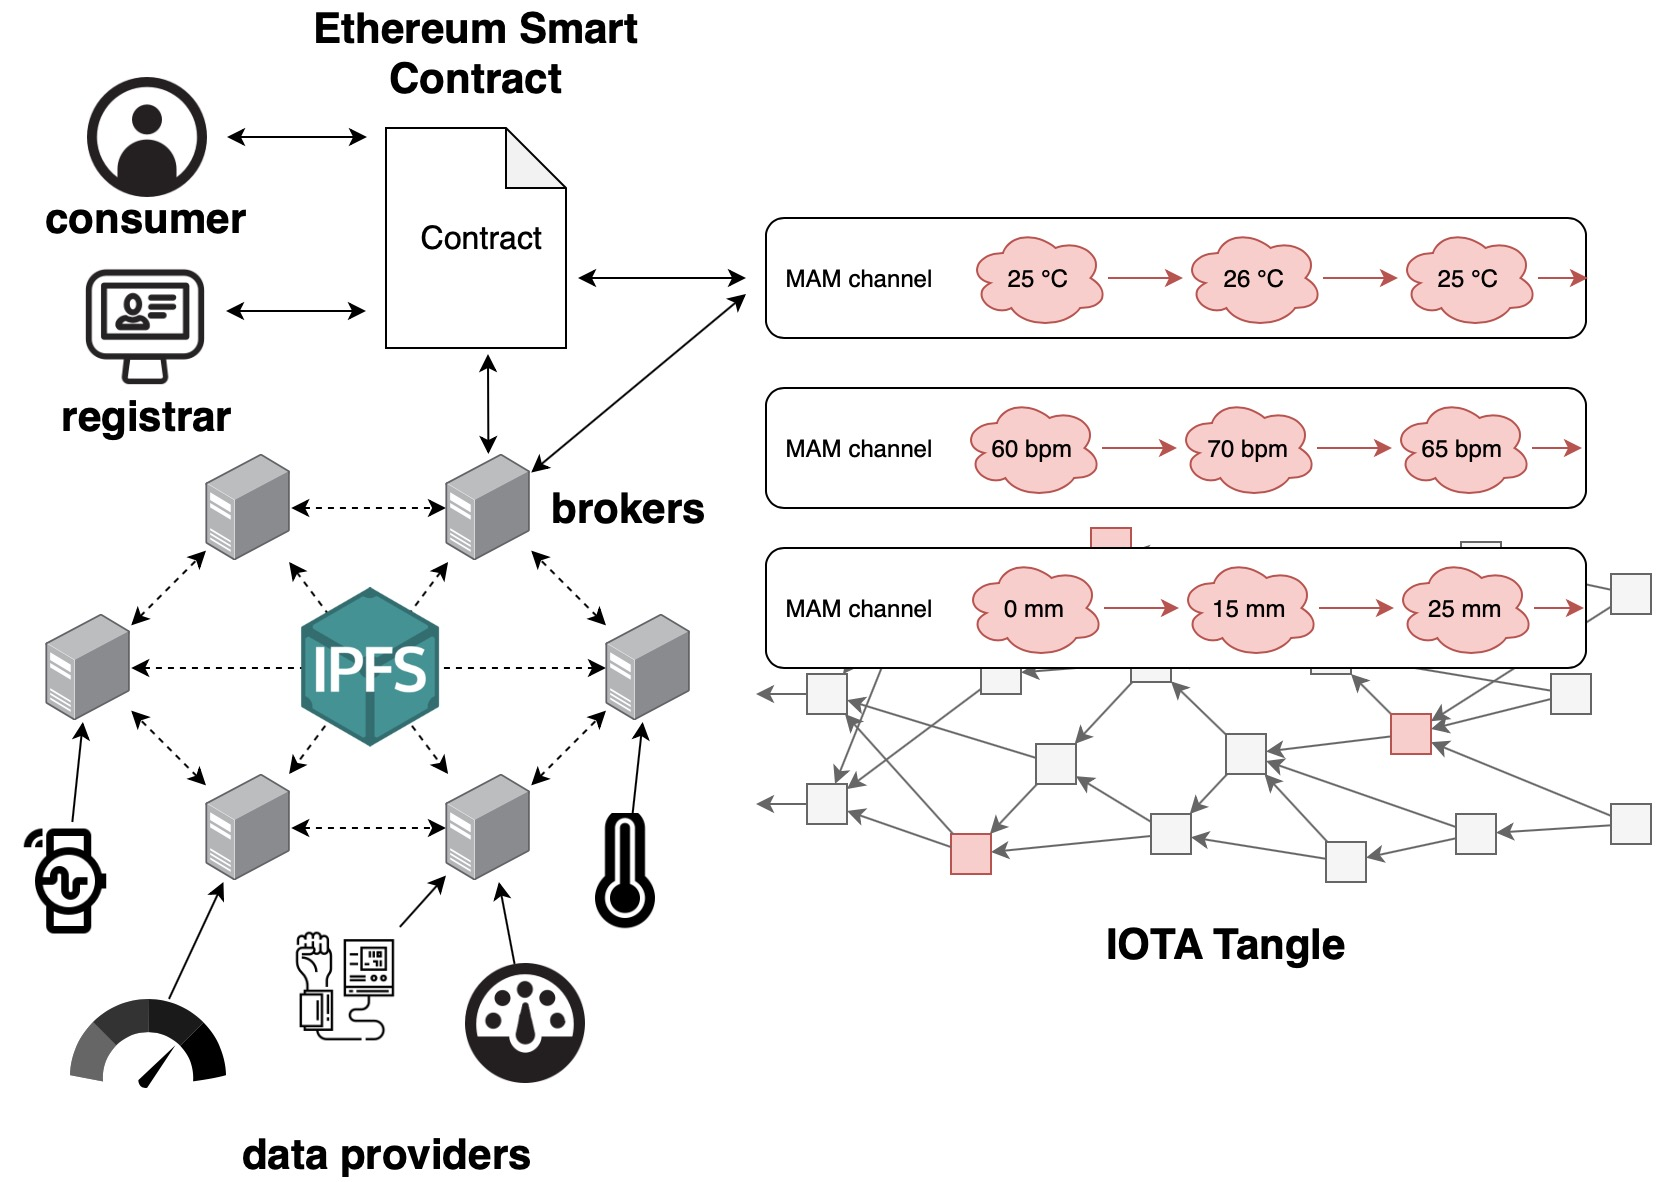
\includegraphics[width=0.4\textwidth]{system_design}
    \caption{The system design of a decentralized architecture which consist of a registrar, data providers, consumers and brokers.}
    \label{fig:system_design}
\end{figure}

\subsection{Components}
\subsubsection{Masked Authenticated Messaging}
IOTA\cite{IOTAwhitepaper} is a feeless and scalable cryptocurrency while MAM is the second layer data communication protocol built on top of Tangle.

MAM resolves the challenge to publish encrypted streaming data to distributed ledgers. It publishes messages encrypted with a \textbf{session key} to the \textbf{channel}, which is a form of transaction where each address can be derived from the previous one. Therefore, with each \textbf{channel root}—the first message of a channel and the session key—all data on the channel is accessible.

One can create multiple channels, however, the size of a channel is fixed which is decided before creation. Thus data providers need to firstly decide how to distribute data product into MAM channels. While the creation of a MAM channel is time-consuming, brokers are also responsible for channel creation, encrypted data publishing and session key certification in our system. See Figure \ref{fig:launching_product}

\begin{figure}[h]
    \centering
    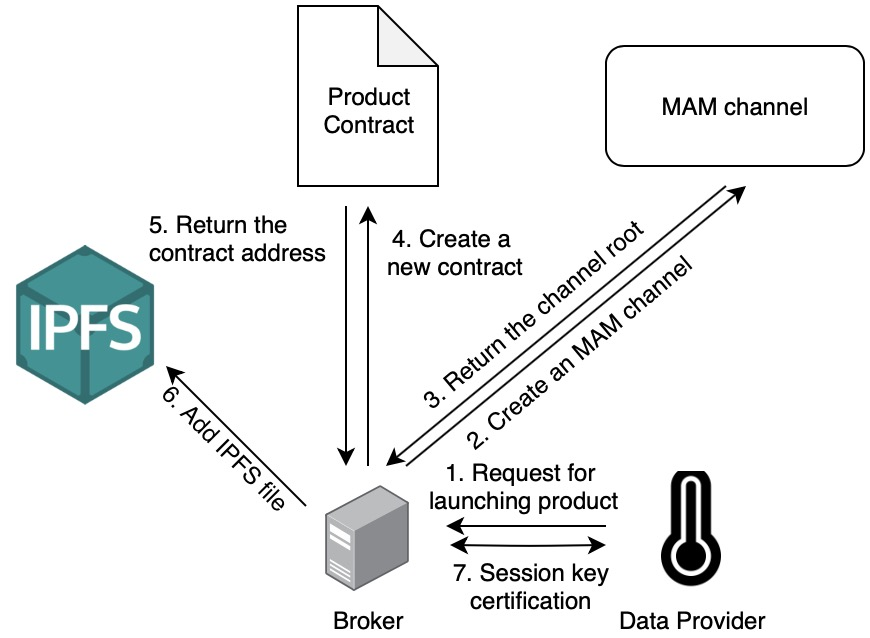
\includegraphics[width=0.4\textwidth]{launching_product}
    \caption{The process of launching a product.}
    \label{fig:launching_product}
\end{figure}

\subsubsection{TangleID}
The TangleID\cite{TangleID} is a self-sovereign identity system based on IOTA that do not require any third-party authority to verify an identity and its digital footprint. With TangleID, the digital footprint is converted into digital assets under the principle of Decentralized Identifiers (DIDs)\cite{DID} defined by W3C. Posting DID documents on MAM makes TangleID a GDPR-Complianced system. Every participant in the data marketplace registers on TangleID, hence one can easily verify data providers' identity to ensure the data persistency from data sources.

\subsubsection{Ethereum Smart Contract}
Smart contract is a protocol for formulating agreement on a blockchain that provides verification and execution of the contract. The code in the smart contract can interact with other contracts, make decisions, store data and transfer cryptocurrency. All conditions and states established in the contract are transparent and with enforcement. The appearance of smart contracts makes trading more flexible, and achieves more complex trading patterns in reality.

\subsubsection{Blind Signature}
There is inherent risk in revealing session keys to brokers since contents may be copied by brokers, which would result in data providers' losses. Therefore, a blind signature is used to prevent session key copying for such circumstances. Blind signature\cite{blindSig} is a form of digital signature where the message is first "blinded" by a random "blinding factor", then passed to a signer to sign. The resulting message, along with the blinding factor, can be later verified with the signer's public key. In our system design, brokers would perform blind signatures during the process of adding new products for data providers, in order to send the secret key of the MAM channel to the smart contract without knowing it.

\subsubsection{IPFS}
Inter-Planetary File system(IPFS)\cite{IPFS} is a peer-to-peer network for storing and accessing files, websites, applications, and data in a distributed file system which is not maintained with certain nodes or entities but is with all IPFS users. In our proposed architecture, brokers are responsible to publish the metadata of products, including title, data provider information and data preview to the IPFS in order to provide users with search capabilities to meet the consumers' need.

\section{\normalsize\textbf{Trading Model}}
In the following, we describe the data trading process in detail where we use game theory to ensure the sustainability of our trading model. To participate a data marketplace, data providers and consumers have to register first. Then data provider can launch its product on the marketplace. Once a product is launched, it is searchable and can be subsequently traded. The whole trading and refunding process is defined in smart contracts which are easily traceable and irreversible.

The consumer will pay for the data, only when the data sold by the data provider sufficiently accurate, for which we called such data "decent data."
Once the accuracy is lower than a certain threshold, which we call "unacceptable data," the consumers would then consider this data provider as a low quality data provider, and stop buying data from this data provider.

Refunds are a major issue in our research. However, we do not need to take refund as a factor in our game theory model, since in our decentralized data marketplace we use a smart contract to store the subscription fee which will be paid to buy the future data. The subscription fee will be paid as new data is transmitted to consumers. In other words, the data provider does not need to perform any procedures to transfer subscription fees from his/her own account to consumers' accounts. For the same reason, data providers have no responsibility on refunding processing fees charged by the smart contract.

\subsection{Participant Registration}
At the beginning, the egistrar creates a registration contract, which maintains all participants' information, including their DID documents and public keys. Anyone can query participants' public keys. Those who would like to sell or purchase data may register to become a data provider or consumer. The registrar has the authority to agree with applications. After that, their identities are available in the registration contract and the launching and trading processes can begin.

\subsection{Launching and Searching Products}
To sell streaming data, a data provider needs to launch a new product on the data marketplace in advance as shown in Figure \ref{fig:launching_product}. The data provider determines a trusted broker and asks the broker to create a new MAM channel and product contract. Each product has a product contract to record the participants, subscription price brokerage fee, quantity of data and  trading process.

Brokers certify session keys as well. Only one session key can be signed in each product, so data providers cannot fake a session key to deceive consumers. Figure \ref{fig:key_certification} shows the certification process. When a data provider asks a broker to certify new session key $k$, the data provider uses the broker's public key, which is available in the Registration Contract after the broker's registration, as a blinding factor, and the session key is blinded. Then the data provider sends the blinded session key $Blind(k)$ to the broker. The broker signs the message and returns the signature $Sign(Blind(k))$ to data provider. The data provider removes the blinding factor and obtains the broker's signature of the session key, $Sign(k)$, which is verifiable by consumers.

\begin{figure}[h]
    \centering
    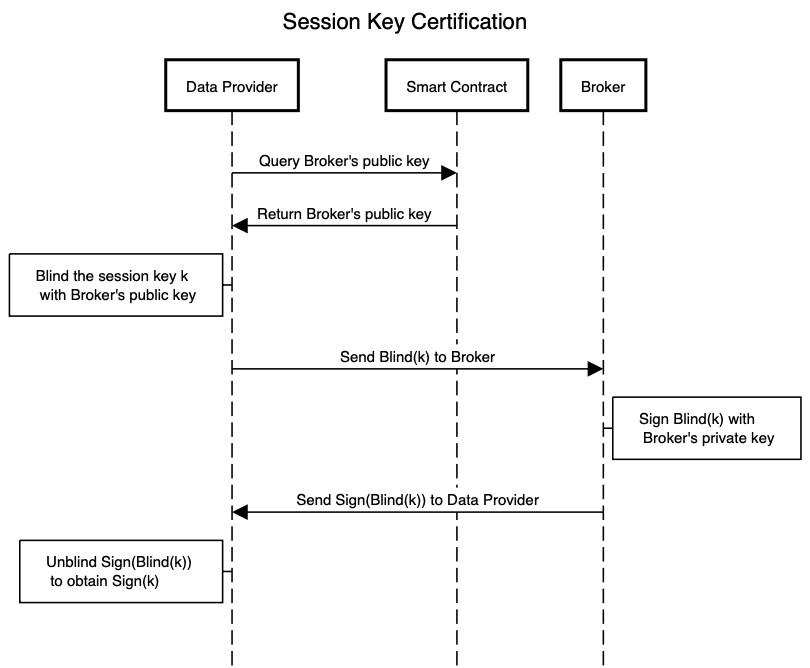
\includegraphics[width=0.5\textwidth]{key_certification}
    \caption{Session key certification process with blind signature.}
    \label{fig:key_certification}
\end{figure}

The contract address and product description will be stored in a file which is uploaded to IPFS. Consumers can search the desired product by keywords or tags. The consumer then evaluates the product and initiates the trading with the data provider if the consumer is interested in subscribing to the data.

\subsection{Trading}
The entire trading process is as shown in Figure \ref{fig:trading_product}. Once a consumer who wants to subscribe certain streaming data that is generated  pays a subscription fee to the product contract, he/she is added to the consumers list automatically by the smart contract.

\begin{figure}[h]
    \centering
    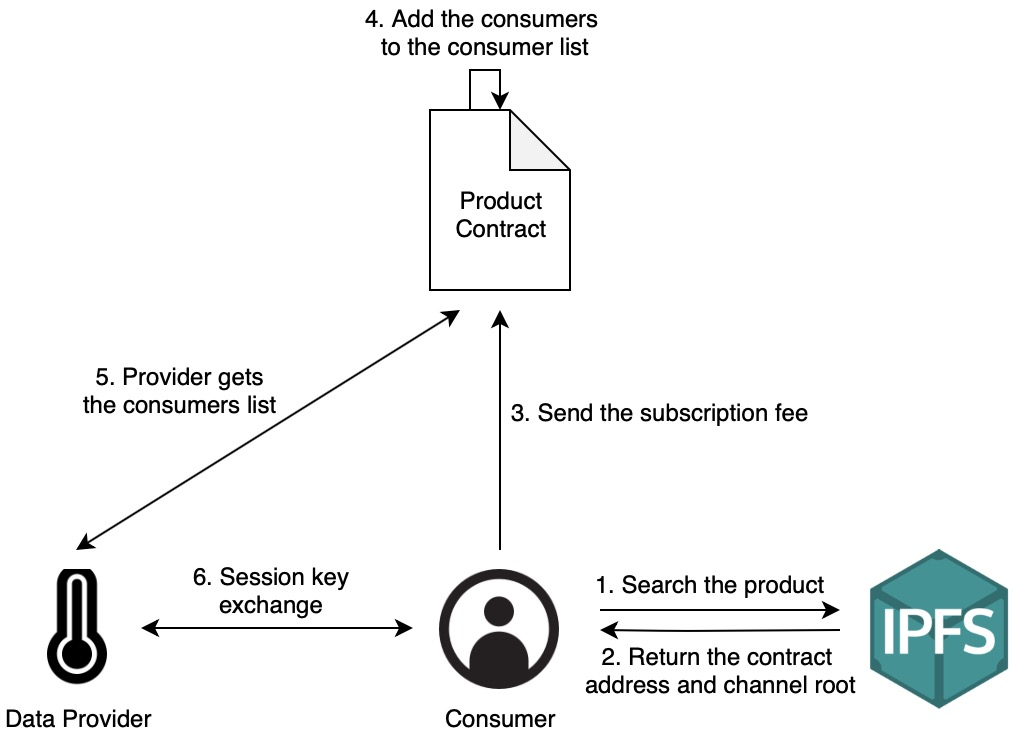
\includegraphics[width=0.4\textwidth]{trading_product}
    \caption{The process for the product trading.}
    \label{fig:trading_product}
\end{figure}

Next, session key $k$ should be exchanged between the data provider and consumers as shown in Figure \ref{fig:key_exchange}. The data provider can obtain public keys of each consumer from the registration contract. For each consumer, the data provider encrypts the session key and broker's signature with the consumer's public key and sends the ciphertext $Encrypt(k + Sign(k))$ to the product contract. Consumers listen to the smart contract event which is triggered when the ciphertext is updated, and decrypt the ciphertext to obtain the session key $k$ and signature $Sign(k)$.

\begin{figure}[h]
    \centering
    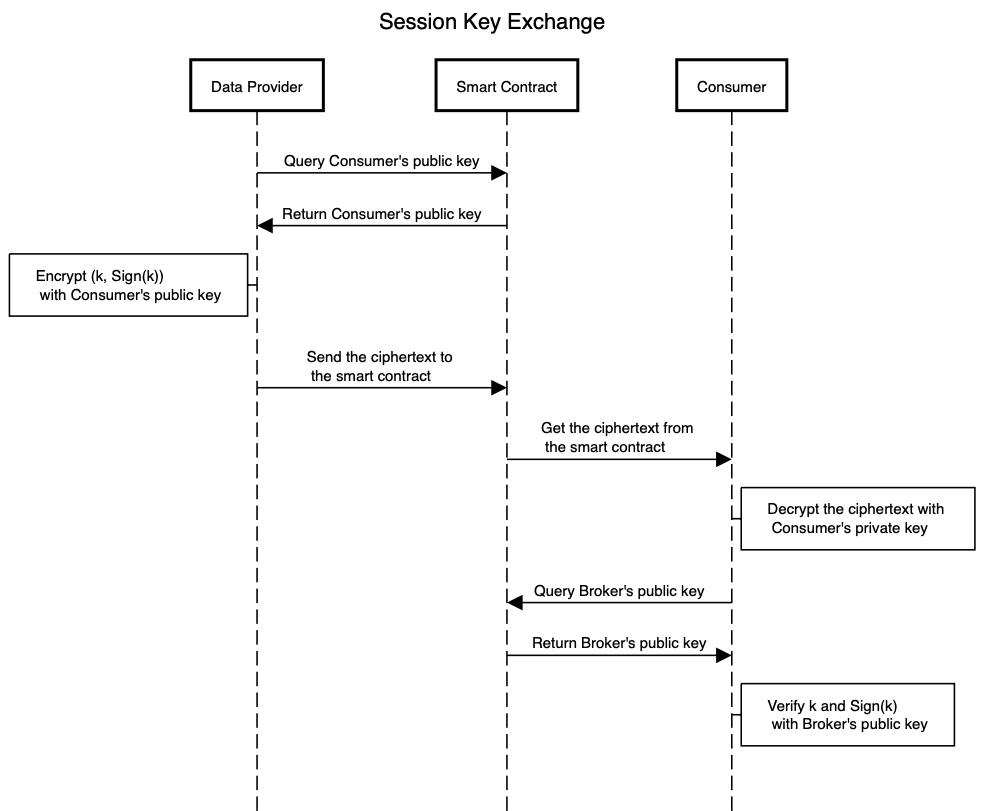
\includegraphics[width=0.5\textwidth]{key_exchange}
    \caption{Session key exchange process between the data provider and consumer.}
    \label{fig:key_exchange}
\end{figure}

Consumers can obtain the broker's public key on the registration contract as well, so they can verify that the signature is valid and the session key is the only one that is certified by the broker. Afterward, encrypted data is published to the MAM channel, and consumers can obtain and decrypt it with the session key.

\subsection{Refunding}
It is probable that the streaming data sources are delayed or even interrupted after the consumers pay the subscription fee. To protect consumer rights, the subscription fee are not transferred to the data provider until data is generated and published to the MAM channel. If the expected data is not available, consumers can request refunds. We assume that a very small percentage of consumers in the product contract are irrational and/or malicious. Each consumer can vote for a refund at any time. If the ratio of consent votes of refunding is higher than the $threshold$ at the $i$th piece of data, the subscription fee is proportionally transferred to the data provider, broker and every consumer. The subscription fee can be prorated as below:

\begin{equation}
    F_{DataProvider}(i) = N price \frac{i-1}{M} (1-F_{b}) -F_{t}
\end{equation}

\begin{equation}
    F_{Broker}(i) = N price \frac{i-1}{M} F_{b} -F_{t}
\end{equation}

\begin{equation}
    F_{Consumer}(i) = price \frac{M-i+1}{M} -F_{t}
\end{equation}

where $price$  is the subscription price, $M$ is the number of expected data samples, $F_{b}$ (\%) is the brokerage fee which is expressed as a percentage, $F_{t}$ is the transaction fee of the smart contract, $N$ is the number of consumers in this contract.

To refund or withdraw subscription fees from the smart contract, the data provider, broker, and consumer send a transaction to execute the smart contract and are responsible for the transaction fee. We assume that only a half of the expected records are published to the MAM channel. When $F_{b}$ is 5\%, the data provider and broker can withdraw half of the total subscription fee from the smart contract and 5\% of the subscription fee belongs to the broker while the remaining belongs to the data provider. For consumers, they can receive half of the subscription fee refunded which should be deducted from the transaction fee.

Considering the situation that one of the consumers requests a refund in the future, when the consumer is disappointed with the data quality, he/she may request a refund.

\subsection{Game Theory Evaluation}
Game Theory is a methodology to discuss strategic interaciton among game players. If we can ensure Nash Equilibrium of decentralized data marketplace exists at a certain acceptable range, then we can promise the sustainability of decentralized data marketplace. Fan Liang et al\cite{SurveyBigDataPricing} listed several different types of game theory models which are applied to data pricing. We employed repeated games to build our game theory model. Repeated games consists of several repetitions of the same base game which meets the scenario of data subscription.

Each consumer would pay subscription fee, $p_s$, each time they receive data from data provider. The sum of all the subscription fee paid to the data provider is denoted as $P_s$.

For every $n$ round, the data provider would pay $C_{maintain}$ to enhance the sensors that the data provider owns. We call this a maintenance period. Moreover, the value of data and the cost of maintenance will decrease as time passes, so we introduce a discounted factor $\beta$ to depict this phenomena.

Following assumptions are made:
\begin{enumerate}
    \item  We assume consumers are rational. \label{rational_man}
    \item  Each data provider is the sole provider of the product they produced. \label{monopoly}
    \item  Subscription fees only depends on data quality. \label{fee_vs_quality}
    \item  At least 51\% of consumers are in the same group which has complete information exchange.\label{51_in_group}
    \item  One of the consumers who has complete information exchange with other 51\% buyers has the ability to examine  data quality. \label{1_in_51}
\end{enumerate}

According to \textbf{assumption(\ref{rational_man})}, we learn that few consumers would take malicious actions in this system, since all the consumers are rational.

\textbf{Assumption(\ref{monopoly})} implies there is no other data providers providing the same product in the data marketplace. In this way, we can consider each provider's behavior independently. That means this decision tree represents the behavior of only one data provider.

From \textbf{assumption(\ref{51_in_group})}, we derive that one of any consumer in that group launches voting for stopping buying data (in other words, the consumer announces the data quality is not acceptable), they would succeed in rejecting the processing subscription.

\textbf{Assumption(\ref{1_in_51})}  implies if unacceptably low accuracy data are delivered to consumers, the examiner will spread this information out.


Based on the description above, the discounted sum of payoff for our repeated game is
\begin{equation} \label{payoff}
    \sum_{i=0}^{m - 1}{\beta^{in}\cdot [(\sum_{j=0}^{n - 1} \beta^j \cdot P_s) - C_{maintain}]}
\end{equation}

Al-Fagih et al. presented\cite{DataPrice} $P_s$ is sigmoid function of $P_r$, and based on rule of thumb $C_{maintain}$ is approximately an exponential function of $P_r$. We can substitute $P_s$ and $C_{maintain}$ with $P_r$ into Eq. (\ref{payoff}), then we can find out the Nash Equilibrium of repeated game.

\subsubsection{Numerical Example}
To evaluate the behavior of the model we presented, first, we would express the function of $P_s$ and $C_{maintain}$ as functions of $P_r$ respectively. Therefore, the sum of subscription fee of all subscriber can be expressed as

\begin{equation} \label{sub_fee}
    P_s = R \frac{e^{a (P_r - b)}}{1 + e^{a (P_r - b)}}
\end{equation}

where $a$ and $b$ are tuning factors, and $R$ is the maximum data value.
And we would express the cost of maintenance as

\begin{equation} \label{C_mtn}
    C_{maintain} = ce^{P_r - d}
\end{equation}
Where $c$ and $d$ are tuning factors.

Substitute Eq. (\ref{sub_fee}) and Eq. (\ref{C_mtn}) into Eq. (\ref{payoff}). We can derive an equation illustrating the market mechanism of the subscription trading policy we used under the decentralized data marketplace. First, data providers have weak motivation to operate their sensor in low accuracy, since the incentive of low quality data is much less than moderate quality data. Second the great deficit at high accuracy is mostly derived by the rapid increasing of maintenance cost. Thus, if the maintenance fee to achieve decent data quality is under a fair price range, then data provider will automatically provide data with high enough data quality under our assumptions.

\section{\normalsize\textbf{Future Work}}
%Data Auction
The data auction process is a data trading mechanism and an economically-driven scheme that establishes corresponding prices of data products through bidding process between consumers and providers. While there has been many auction models\cite{BigPicDataMarket} in several areas, there has been minimal research on third-party auction platforms. Our proposed decentralized data marketplace protects the privacy of participants which reveals the minimum information for validation and reduces the suspicion of trust to centralized parties or auctioneers. However, the auction process between multiple participants and analysis of potential threats are still critical issues that need to be resolved. For the game theory model presented in this work, we assume each data provider's behavior is independent. However, normally there would be multiple data providers providing similar products (substitutions). Only one provider is taken into considerations at present.


% ---- Bibliography ----
\bibliographystyle{IEEEtran}
\bibliography{references}
\end{document}
